\subsection{Remote Desktop}
\begin{frame}[fragile]{Connecting: Remote Desktop}
\begin{itemize}
\item First time starting a remote desktop:
\begin{semiverbatim}
\footnotesize
[sjr20@{\color{red}login-sand2} ~]\$ vncserver

You will require a password to access your desktops.

Password: 
Verify:   
Would you like to enter a view-only password (y/n)? n

New 'X' desktop is {\color{red}login-sand2:8}

Starting applications specified in /home/sjr20/.vnc/xstartup.turbovnc
Log file is /home/sjr20/.vnc/login-sand2:8.log
\end{semiverbatim}
\smallskip\item<2->\alert{For 3D graphics sessions, use {\color{red}login-gfx1} or {\color{red}login-gfx2}.}
\end{itemize}
\end{frame}

\begin{frame}[fragile]{Connecting: Remote Desktop}
\begin{itemize}
\item Remote desktop already running:
\begin{semiverbatim}
\footnotesize
[sjr20@login-sand2 ~]\$ vncserver -list

TurboVNC server sessions:

X DISPLAY #     PROCESS ID
:8              12745
\end{semiverbatim}
\smallskip\item Kill it:
\begin{semiverbatim}
\footnotesize
[sjr20@login-sand2 ~]\$ vncserver -kill :8
Killing Xvnc process ID 12745
\end{semiverbatim}
\smallskip\item\alert{Typically you only need {\color{red}one} remote desktop.}
\item\alert{Keeps running until killed, or the node reboots.}
\end{itemize}
\end{frame}

\begin{frame}[fragile]{Connecting: Remote Desktop}
\begin{itemize}
\item To connect to the desktop from Linux:
\begin{semiverbatim}
\scriptsize
[sjr20@themis ~]\$ vncviewer -via sjr20@{\color<2->{red}login-sand2}.hpc.cam.ac.uk localhost:{\color<2->{red}8}
Connected to RFB server, using protocol version 3.8
Enabling TightVNC protocol extensions
Performing standard VNC authentication
Password:
\end{semiverbatim}
\smallskip
\item{\alert{Press F8 to bring up the control panel.}}
\pause
\item{Exercise 3 - Remote desktop}
\end{itemize}
\end{frame}

\begin{frame}{HPCS TurboVNC Session}
\begin{center}
\centerline{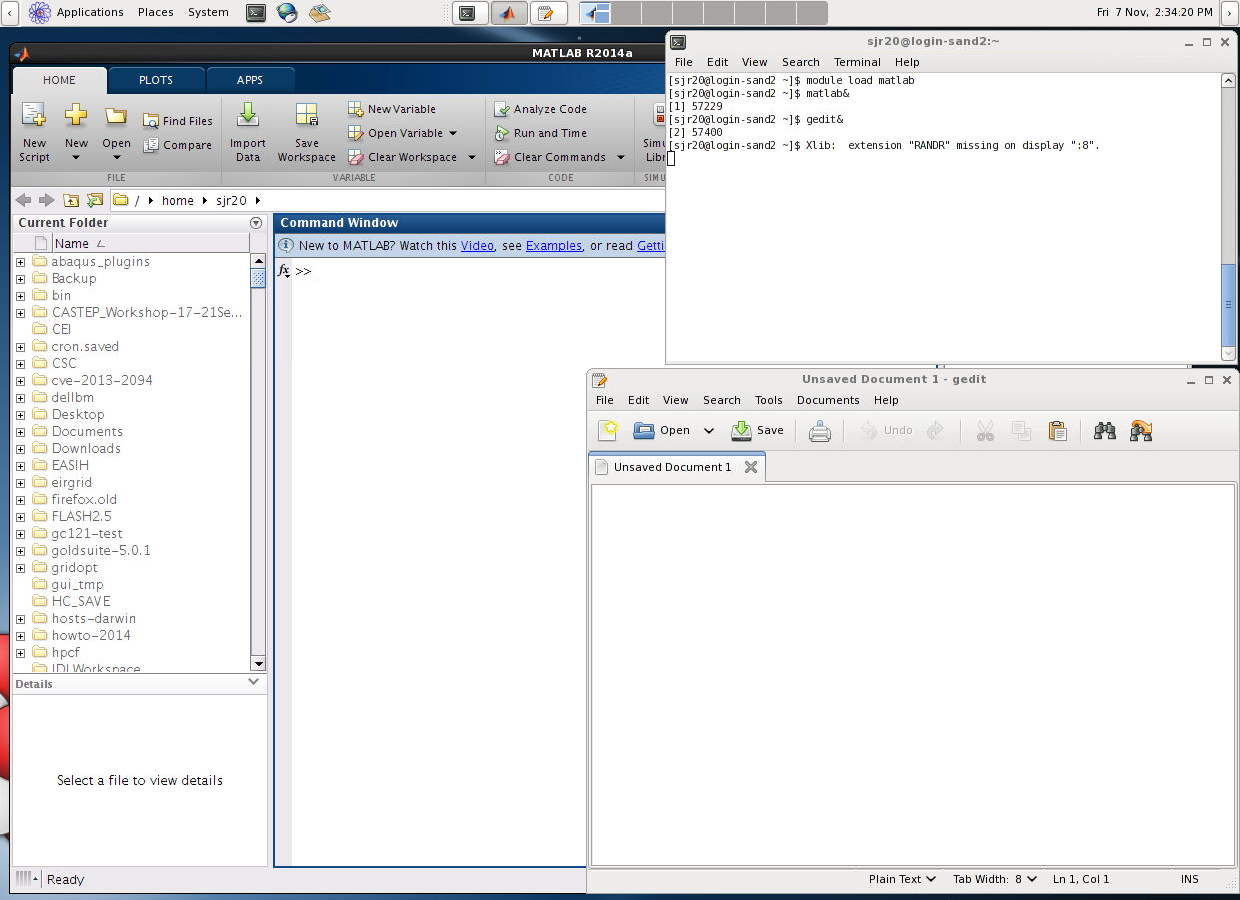
\includegraphics[width=0.85\textwidth]{imgs/linux-turbovnc.png}}
\end{center}
\end{frame}

\begin{frame}{Linux TurboVNC Control Panel}
\begin{center}
\centerline{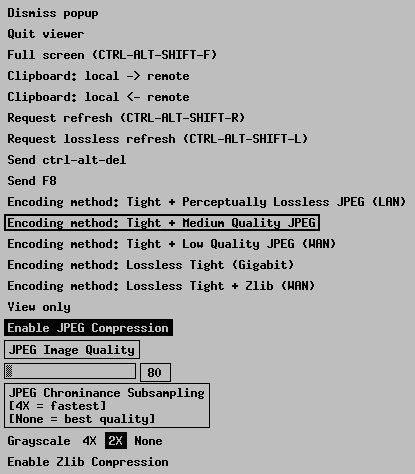
\includegraphics[height=0.8\textheight]{imgs/linux-turbovnc-F8.png}}
\end{center}
\end{frame}

\begin{frame}{Connecting: Remote Desktop (MobaXterm)}
\begin{center}
\centerline{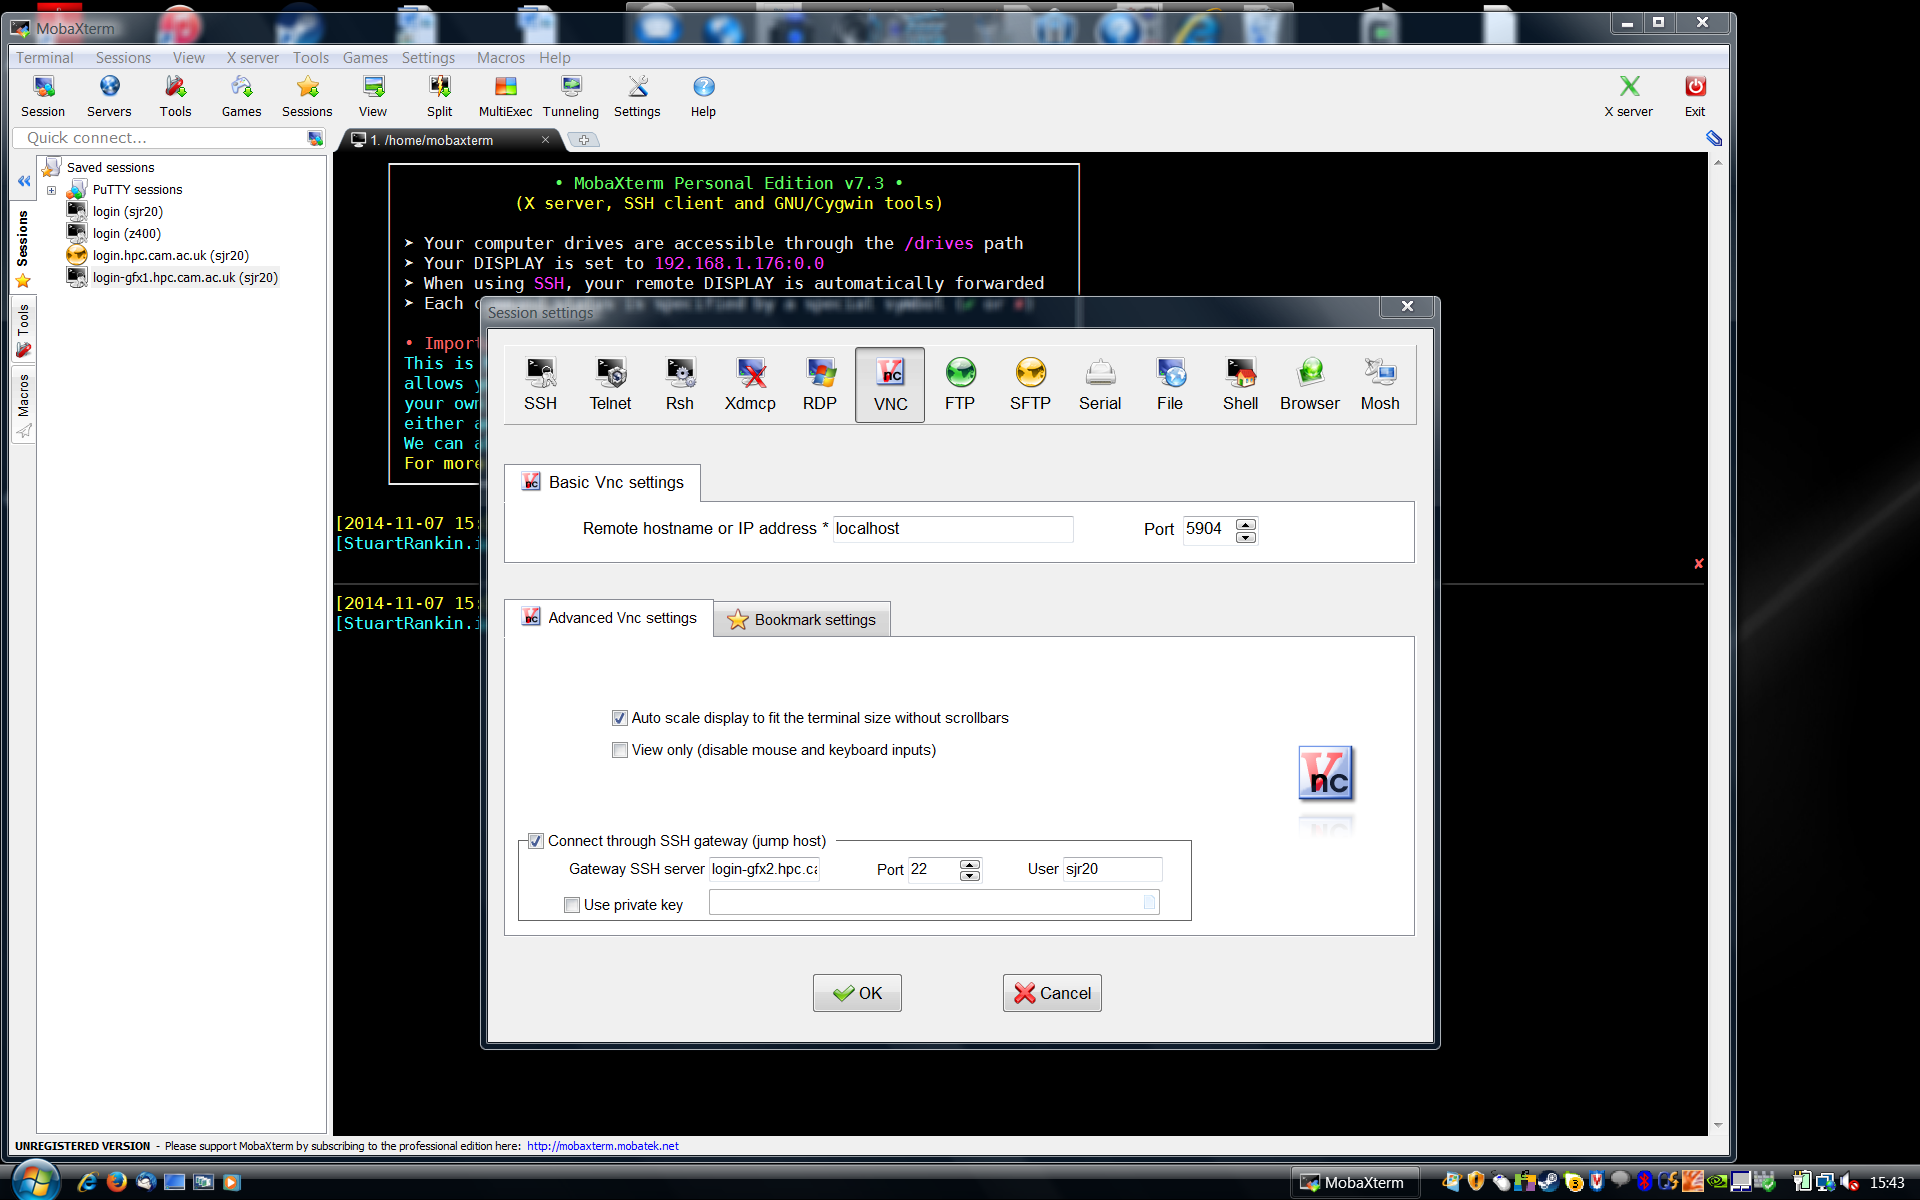
\includegraphics[height=0.8\textheight]{imgs/mobaxterm-turbovnc.png}}
\end{center}
\end{frame}

\begin{frame}{Connecting: Remote Desktop (MobaXterm)}
\begin{center}
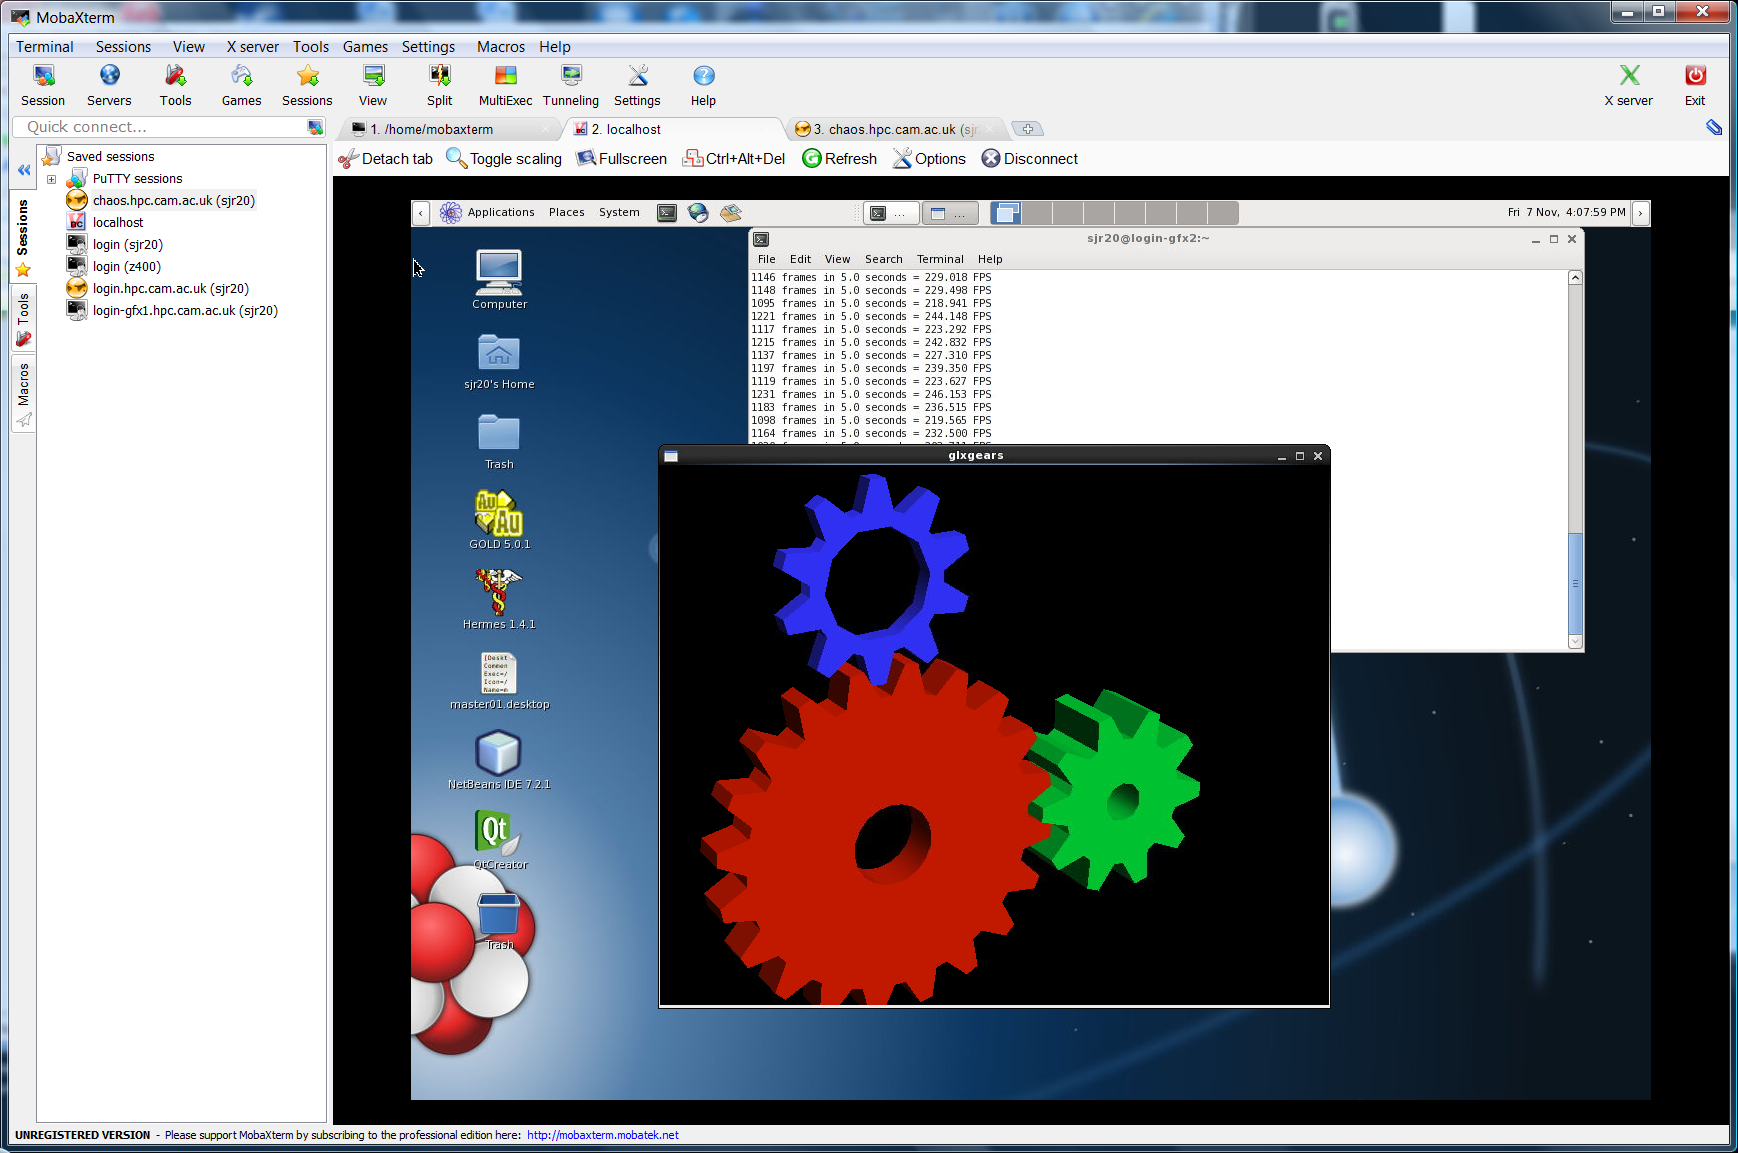
\includegraphics[height=0.8\textheight]{imgs/mobaxterm-vgl-turbovnc.png}
\end{center}
\end{frame}

\begin{frame}{3D Remote Visualization}
\begin{center}
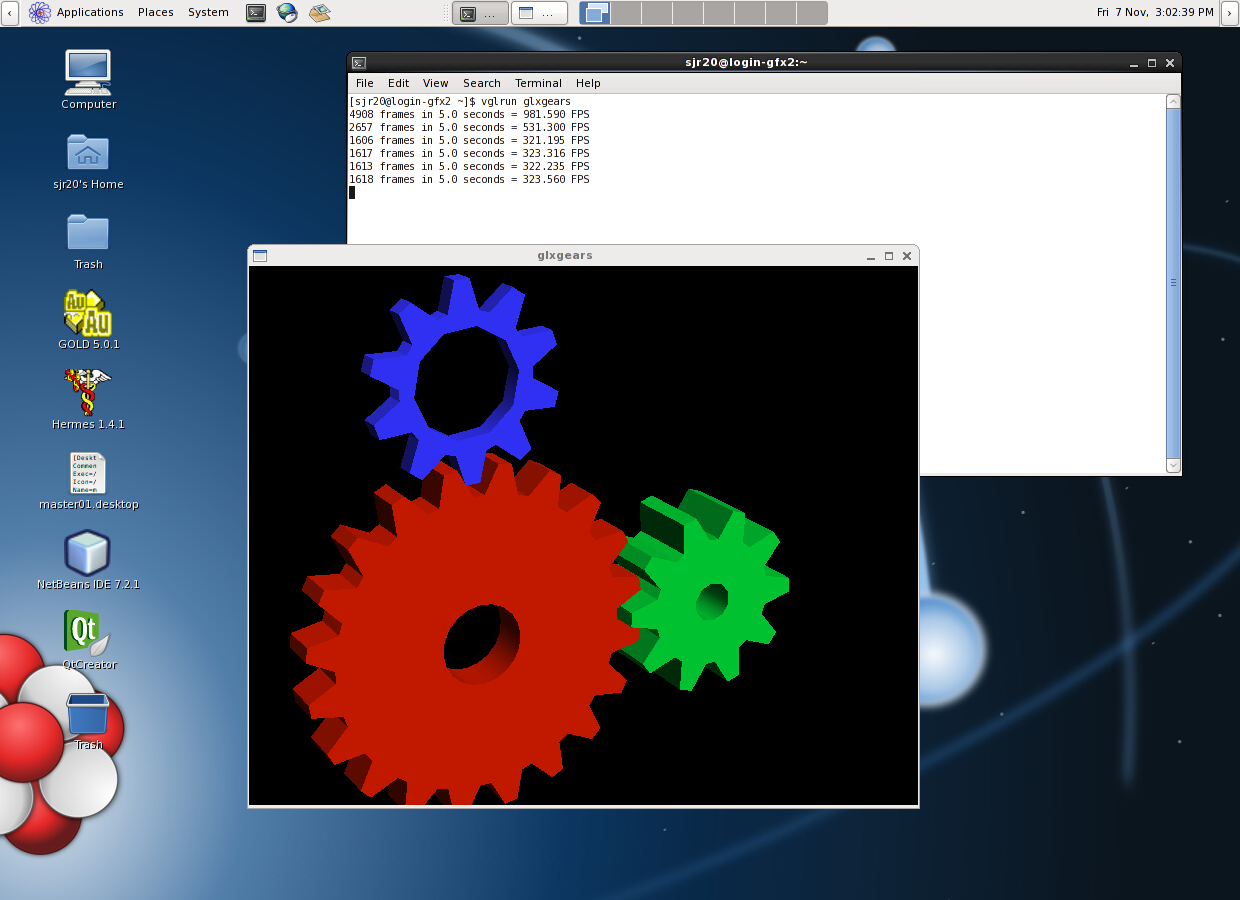
\includegraphics[height=0.8\textheight]{imgs/vgl-turbovnc.png}
\end{center}
\end{frame}

\begin{frame}{3D Remote Visualization}
\begin{itemize}
\item{Choose \alert{login-gfx2}.}
\item{Launch any application requiring 3D (OpenGL) with \alert{vglrun}.}
\item{May need to adjust the compression level for your network connection.}
\end{itemize}
\end{frame}